\documentclass[11pt]{article}
\usepackage{fullpage}
\usepackage{amsmath,amsthm,amssymb,amsfonts,multirow}
\usepackage{mathtools}
\usepackage{graphicx}
\usepackage{xcolor}
\usepackage{float}
%\usepackage{enumerate}
\usepackage[shortlabels, inline]{enumitem}
\usepackage{textcomp}
\usepackage{hyperref}
\usepackage{comment}

\usepackage{listings}
\lstset{language=Python, numbers=left, basicstyle=\ttfamily, keywordstyle=\color{blue}, showstringspaces=false}

\usepackage[style=alphabetic-verb]{biblatex}
% \bibliography{Problems/ref.bib}

\newcommand{\N}{\mathbb{N}}
\newcommand{\Z}{\mathbb{Z}}
\newcommand{\Q}{\mathbb{Q}}
\newcommand{\R}{\mathbb{R}}
\newcommand{\C}{\mathcal{C}}
\newcommand{\K}{\mathbb{K}}
\renewcommand{\div}{\mid}
\newcommand{\ndiv}{\nmid}
\newcommand{\E}{\mathbb{E}}
\newcommand{\I}{\mathbb{I}}
\newcommand{\F}{\mathcal{F}}

\DeclareMathOperator{\id}{Id}
\DeclareMathOperator{\tr}{Tr}
\DeclareMathOperator*{\argmax}{arg\,max}
\DeclareMathOperator*{\argmin}{arg\,min}
\DeclareMathOperator{\lcm}{lcm}
\DeclareMathOperator{\spn}{span}
\DeclareMathOperator{\acosh}{acosh}

\DeclarePairedDelimiter{\floor}{\lfloor}{\rfloor}
\DeclarePairedDelimiter{\ceil}{\lceil}{\rceil}
\DeclarePairedDelimiter{\abs}{\lvert}{\rvert}

\newcommand{\subtag}[1]{\tag{\theparentequation#1}}

\renewcommand{\vec}[1]{\mathbf{#1}}

\usepackage{subfiles}
\usepackage{subcaption}
\makeatletter
\newcommand\nocaption{
    \renewcommand\p@subfigure{}
    \renewcommand{\thesubfigure}{\arabic{figure}\alph{subfigure}}
}
\makeatother


\newenvironment{problem}[2][Question]{\begin{trivlist}
\item[\hskip \labelsep {\bfseries #1}\hskip \labelsep {\bfseries #2.}]}{\end{trivlist}}

\newenvironment{solution}{%
  \begin{proof}[\textbf{Solution}]$ $\par\nobreak\ignorespaces
}{%
  \end{proof}
}

\theoremstyle{definition}
\newtheorem{definition}{Definition}
\newtheorem{theorem}{Theorem}
\newtheorem{lemma}{Lemma}

\hypersetup{
    colorlinks=true,
    linkcolor=blue,
    filecolor=magenta,      
    urlcolor=cyan,
    pdftitle={Overleaf Example},
    pdfpagemode=FullScreen,
    }


\title{Intro to Computational Mathematics: Section 11}
\date{November 2025}

\begin{document}
\maketitle

\begin{problem}{6.4.1}
For each IVP, write out (possibly using a calculator) the first time step of the improved Euler method with $h = 0.2$.
\begin{enumerate}[(a)]
    \item $u' = -2tu$, $0 \leq t \leq 2$, $u(0) = 2$; $\hat{u}(t) = 2e^{-t}$
    \item $u' = u + t$, $0 \leq t \leq 1$, $u(0) = 2$; $\hat{u}(t) = -1 -t + 3e^t$
    \item $(1 + x^3)uu' = x^2$, $0 \leq x \leq u$, $u(0) = 1$; $\hat{u}(x) = [1 + (2/3)\ln(1 + x^3)]^{1/2}$
\end{enumerate}
\end{problem}
\begin{solution}
The improved Euler method takes steps of the form: $$u_{i+1} = u_i + h \cdot f\left(t_i + \frac{1}{2}h, u_i + \frac{1}{2}h f(t_i, u_i)\right).$$ Expressing this for the systems given:
\begin{align*}
    u(0.2) &= u(0) + (0.2)\cdot f\left(0 + \frac{1}{2}(0.2), u(0) + \frac{1}{2}(0.2)f(0, u(0)) \right) \\
    u(0.2) &= u(0) + (0.2)\cdot f\left(0.1 , u(0) + (0.1)f(0, u(0)) \right) \\
\end{align*}

\begin{enumerate}[(a)]
    \item
    \begin{align*}
        u(0.2) &= 2 + (0.2)\cdot f\left(0.1 , 2 + (0.1)(-2(0)(2)) \right) \\
        &= 2 + (0.2)\cdot f\left(0.1 , 2 \right) \\
        &= 2 + (0.2)\cdot (-2(0.1)(2)) \\
        &= 1.92
    \end{align*}
    \item
    \begin{align*}
        u(0.2) &= 2 + (0.2)\cdot f\left(0.1 , 2 + (0.1)(2 + 0) \right) \\
        &= 2 + (0.2)\cdot f\left(0.1 , 2.2 \right) \\
        &= 2 + (0.2)(0.1 + 2.2) \\
        &= 2.46
    \end{align*}
    \item We need to rewrite this problem in a form that we can use:
    $$u' = \frac{x^2}{(1 + x^3)u}.$$
    \begin{align*}
        u(0.2) &= 1 + (0.2)\cdot f\left(0.1 , 1 + (0.1)\left(\frac{0^2}{(1 + (0)^3)(1)}\right) \right) \\
        &= 1 + (0.2)\cdot f\left(0.1 , 1 \right) \\
        &= 1 + (0.2)\cdot \frac{(0.1)^2}{(1 + (0.1)^3)(1)} \\
        &= 1.00199800199
    \end{align*}
\end{enumerate}
\end{solution}



\begin{problem}{6.4.2}
Use the modified Euler method to solve the problems in \href{https://fncbook.com/rk/#problem-rk-byhand}{Exercise 6.4.1}.
\end{problem}
\begin{solution}
The butcher table for the modified Euler method (ME2) is:
\begin{center}
    \begin{tabular}{c|cc}
    0 & & \\
    1 & 1 & \\\hline
    & $\frac{1}{2}$ & $\frac{1}{2}$
    \end{tabular}
\end{center}
This table can be interpreted into the RK type system as:
\begin{align*}
    k_1 &= h f(t_i, u_i) \\
    k_2 &= h f(t_i + (1)h, u_i + (1)k_1) \\
    &= f(t_i + h, u_i + k_1) \\
    u_{i+1} &= u_i + (1)k_1 + (1)k_2 \\
    &= u_i + (\frac{1}{2})k_1 + (\frac{1}{2})k_2
\end{align*}
Plugging in for each problem:
\begin{enumerate}[(a)]
    \item
    \begin{align*}
        k_1 &= (0.2) f(0, 2) \\
        &= (0.2) \cdot -2(0)(2) \\
        &= 0 \\
        k_2 &= (0.2) f(0 + 0.2, 2 + 0) \\
        &= (0.2) f(0.2, 2) \\
        &= (0.2) \cdot -2(0.2)(2) \\
        &= -0.16 \\
        u(0.2) &= 2 + (\frac{1}{2})0 - (\frac{1}{2})0.16 \\
        &= 1.92
    \end{align*}
    \item
    \begin{align*}
        k_1 &= (0.2) f(0, 2) \\
        &= (0.2) (2 + 0) \\
        &= 0.4 \\
        k_2 &= (0.2) f(0 + 0.2, 2 + 0.4) \\
        &= (0.2) f(0.2, 2.4) \\
        &= (0.2) (2.4 + 0.2) \\
        &= 0.52 \\
        u(0.2) &= 2 + (\frac{1}{2})0.4 + (\frac{1}{2})0.52 \\
        &= 2.46
    \end{align*}
    \item
    \begin{align*}
        k_1 &= (0.2) f(0, 1) \\
        &= (0.2) \frac{0^2}{(1 + (0)^3)(1)} \\
        &= 0 \\
        k_2 &= (0.2) f(0 + 0.2, 1 + (0)) \\
        &= (0.2) f(0.2, 1) \\
        &= (0.2) \frac{(0.2)^2}{(1 + (0.2)^3)(1)} \\
        &= 0.00793650793 \\
        u(0.2) &= 1 + (\frac{1}{2})0 + (\frac{1}{2})0.00793650793 \\
        &= 1.00396825396
    \end{align*}
\end{enumerate}
\end{solution}



\begin{problem}{6.4.3}
Modify \href{https://fncbook.com/rk/#function-rk4}{Function 6.4.2} to implement the modified Euler method. Test your function on the IVP in part (a) of \href{https://fncbook.com/rk/#problem-rk-byhand}{Exercise 6.4.1} by solving with $n = 30, 60, 90, \ldots, 300$ and plotting the convergence of the error at the final time together with a line showing $O(n^{-2})$.
\end{problem}
\begin{solution}
The following code computes the solution for both 6.4.3 and 6.4.5 simultaneously:
\begin{lstlisting}
import numpy as np
import matplotlib.pyplot as plt

def me2(du_dt, tspan, u0, n):
    # Time discretization.
    a, b = tspan
    h = (b - a) / n
    t = np.linspace(a, b, n + 1)

    # Initialize output.
    u = np.zeros((n + 1, len(np.atleast_1d(u0))))
    u[0] = u0

    # Time stepping.
    for i in range(n):
        k1 = h * du_dt(t[i], u[i])
        k2 = h * du_dt(t[i] + h, u[i] + k1)
        u[i + 1] = u[i] + 0.5*k1 + 0.5*k2
    return t, u.T


def heun(du_dt, tspan, u0, n):
    # Time discretization.
    a, b = tspan
    h = (b - a) / n
    t = np.linspace(a, b, n + 1)

    # Initialize output.
    u = np.zeros((n + 1, len(np.atleast_1d(u0))))
    u[0] = u0

    # Time stepping.
    for i in range(n):
        k1 = h * du_dt(t[i], u[i])
        k2 = h * du_dt(t[i] + (2/3)*h, u[i] + (2/3)*k1)
        u[i + 1] = u[i] + (1/4)*k1 + (3/4)*k2
    return t, u.T

def f(t, u):
    return -2*t*u

def soln(t):
    return 2 * np.exp(-t**2)

n = [i for i in range(30, 301, 30)]
t = []
err_me2 = []
err_heun = []
for n_ in n:
    t, U_n = me2(f, [0, 2], 2, n_)
    U_n = U_n.flatten()
    err_me2.append(abs(soln(t[-1]) - U_n[-1]))

    t, U_n = heun(f, [0, 2], 2, n_)
    U_n = U_n.flatten()
    err_heun.append(abs(soln(t[-1]) - U_n[-1]))

plt.plot(n, err_me2, label='ME2')
plt.plot(n, err_heun, label='Heun')
n_ = np.linspace(30, 301, 400)
plt.plot(n_, [i**(-2) for i in n_], label='$n^{-2}$')
plt.legend()
plt.yscale('log')
plt.xscale('log')

plt.title('Comparison of RK type Methods')
plt.show()
\end{lstlisting}
Ouptut:
\begin{center}
    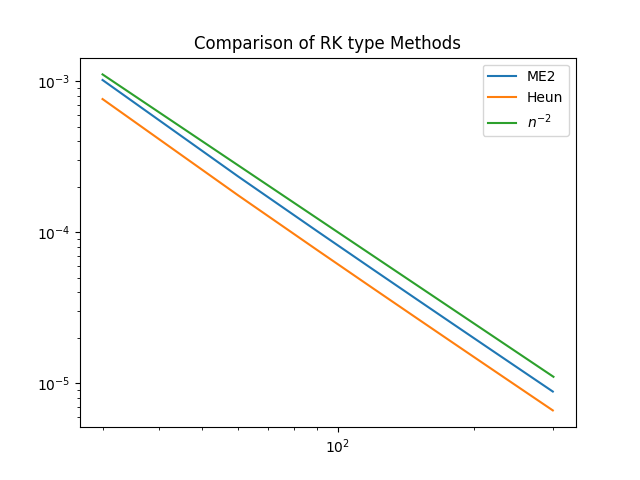
\includegraphics[width=0.8\textwidth]{6.4.3_5_fig.png}
\end{center}
\end{solution}



\begin{problem}{6.4.4}
Use Heun's method to solve the problems in \href{https://fncbook.com/rk/#problem-rk-byhand}{Exercise 6.4.1}.
\end{problem}
The butcher table for Heun's method is:
\begin{center}
    \begin{tabular}{c|cc}
    0 & & \\
    $\frac{2}{3}$ & $\frac{2}{3}$ & \\\hline
    & $\frac{1}{4}$ & $\frac{3}{4}$
    \end{tabular}
\end{center}
This table can be interpreted into the RK type system as:
\begin{align*}
    k_1 &= h f(t_i, u_i) \\
    k_2 &= h f(t_i + \frac{2}{3}h, u_i + \frac{2}{3}k_1) \\
    u_{i+1} &= u_i + \frac{1}{4}k_1 + \frac{3}{4}k_2 \\
\end{align*}
Plugging in for each problem:
\begin{enumerate}[(a)]
    \item
    \begin{align*}
        k_1 &= (0.2) f(0, 2) \\
        &= (0.2) \cdot (-2(0)(2)) \\
        &= 0 \\
        k_2 &= (0.2) f(0 + \frac{2}{3}(0.2), 2 + \frac{2}{3}(0)) \\
        &= (0.2) f(\frac{2}{15}, 2) \\
        &= (0.2) \cdot (-2(\frac{2}{15})(2)) \\
        &= -\frac{16}{15} \\
        u(0.2) &= 2 + \frac{1}{4}(0) + \frac{3}{4}(-\frac{8}{75})\\
        &= 1.92
    \end{align*}
    \item
    \begin{align*}
        k_1 &= (0.2) f(0, 2) \\
        &= (0.2) \cdot (2 + 0) \\
        &= 0.4 \\
        k_2 &= (0.2) f(0 + \frac{2}{3}(0.2), 2 + \frac{2}{3}(0.4)) \\
        &= (0.2) f(\frac{2}{15}, \frac{34}{15}) \\
        &= (0.2) \cdot (\frac{34}{15} + \frac{2}{15}) \\
        &= \frac{12}{25} \\
        u(0.2) &= 2 + \frac{1}{4}(\frac{2}{5}) + \frac{3}{4}(\frac{12}{25}) \\
        &= 2.46
    \end{align*}
    \item
    \begin{align*}
        k_1 &= (0.2) f(0, 1) \\
        &= (0.2) \frac{0^2}{(1 + (0)^3)(1)} \\
        &= (0.2) 0 \\
        k_2 &= (0.2) f(0 + \frac{2}{3}(0.2), 1 + \frac{2}{3}(0)) \\
        &= (0.2) f(\frac{2}{15}, 1) \\
        &= (0.2) \frac{(\frac{2}{15})^2}{(1 + (\frac{2}{15})^3)(1)} \\
        &= 0.0035471475 \\
        u(0.2) &= 1 + \frac{1}{4}(0) + \frac{3}{4}(0.0035471475) \\
        &= 1.00266036062
    \end{align*}
\end{enumerate}
\begin{solution}
\end{solution}



\begin{problem}{6.4.5}
Modify \href{https://fncbook.com/rk/#function-rk4}{Function 6.4.2} to implement Heun's method. Test your function on the IVP in part (a) of \href{https://fncbook.com/rk/#problem-rk-byhand}{Exercise 6.4.1} by solving with $n = 30, 60, 90, \ldots, 300$ and plotting the convergence of the error at the final time together with a line showing $O(n^{-2})$.
\end{problem}
\begin{solution}
    See solution to 6.4.3 above.
\end{solution}



\begin{problem}{Q2}
Consider the following initial value problem given by a system of two first-order differential equations
$$
\begin{bmatrix}
    \frac{d}{dt} x(t)\\ \frac{d}{dt} y(t) 
\end{bmatrix} = \begin{bmatrix}
    -y(t)\\ x(t) 
\end{bmatrix}
$$
with initial condition $x(0)=1$ and $y(0)=0$. Note the true solution to this system of equations is $\hat x(t)=\cos(t)$ and $\hat y(t) = \sin(t)$ (geometrically, this just spins counter-clockwise).\\

\noindent {\bf (a)}
State an upper bound on how different Euler's method with a generic stepsize $h>0$ can be from the true solution at a generic time $t>0$. \\ 
Calculate and plot the trajectory of Euler's method with $h=1$ for two steps.

\vskip 3cm


\noindent {\bf (b)} State an upper bound on how different the Improved Euler's method with a generic stepsize $h>0$ can be from the true solution at a generic time $t>0$. \\
Calculate and plot the trajectory of the Improved Euler's method with $h=1$ for two steps.
\end{problem}
\begin{solution}
\begin{enumerate}[(a)]
\item An upper bound on the error of Euler's method can be given by the global error formula: $$\|\hat{u}(t_i) - u_i\| \leq \frac{Ch^p}{L}\left[e^{\|L(t_i - a)\|} - 1\right].$$ To give a slightly more exact bound on error for this problem, we need to bound the constants. Euler's method has $\tau(h) \approx \frac{h}{2} \hat{u}'' + O(h^2)$. A reasonable upper bound then is to take the $\|\hat{u}''\|_\infty = \left\|\begin{bmatrix*}-\cos(t) \\ -\sin(t)\end{bmatrix*}\right\|_\infty\leq 1$. With Euler's method, we can take $p = 1$. The next constant we need to bound is $L$. To do so, we need to express $\phi$ in terms of $u$ and $t$:
$$\begin{bmatrix*}\dot{x}(t) \\ \dot{y}(t)\end{bmatrix*} = \begin{bmatrix*}0 & -1 \\ 1 & 0\end{bmatrix*}\begin{bmatrix*}x(t) \\ y(t)\end{bmatrix*}.$$
Using this expression, we can now give a value for $L$ as $\left\|\frac{\partial \phi}{\partial u}(t_i, u_i, h)\right\|_\infty = \left\|\begin{bmatrix*}0 & -1 \\ 1 & 0\end{bmatrix*}\right\|_\infty = 1$. So letting $L = 1$ is a reasonable choice.
Since $a = \begin{bmatrix*}0 \\ 0\end{bmatrix*}$, we write down the following upper bound on the global error:
$$\|\hat{u}(t_i) - u_i\|_\infty \leq h\left[e^{\left\|t_i - \begin{bmatrix*}0 \\ 0\end{bmatrix*}\right\|_{\infty}} - 1\right].$$

Our approximation of $u$ from the two steps of Euler's method:
\begin{align*}
    \begin{bmatrix*}x(1) \\ y(1)\end{bmatrix*} &= \begin{bmatrix*}x(0) \\ y(0)\end{bmatrix*} + (1)\begin{bmatrix*}0 & -1 \\ 1 & 0\end{bmatrix*}\begin{bmatrix*}x(0) \\ y(0)\end{bmatrix*} \\
    &= \begin{bmatrix*}1 \\ 0\end{bmatrix*} + (1)\begin{bmatrix*}0 & -1 \\ 1 & 0\end{bmatrix*}\begin{bmatrix*}1 \\ 0\end{bmatrix*} \\
    &= \begin{bmatrix*}1 \\ 1\end{bmatrix*} \\
    \begin{bmatrix*}x(2) \\ y(2)\end{bmatrix*} &= \begin{bmatrix*}x(1) \\ y(1)\end{bmatrix*} + (1)\begin{bmatrix*}0 & -1 \\ 1 & 0\end{bmatrix*}\begin{bmatrix*}x(1) \\ y(1)\end{bmatrix*} \\
    &= \begin{bmatrix*}1 \\ 1\end{bmatrix*} + (1)\begin{bmatrix*}0 & -1 \\ 1 & 0\end{bmatrix*}\begin{bmatrix*}1 \\ 1\end{bmatrix*} \\
    &= \begin{bmatrix*}0 \\ 2\end{bmatrix*}
\end{align*}
\begin{center}
    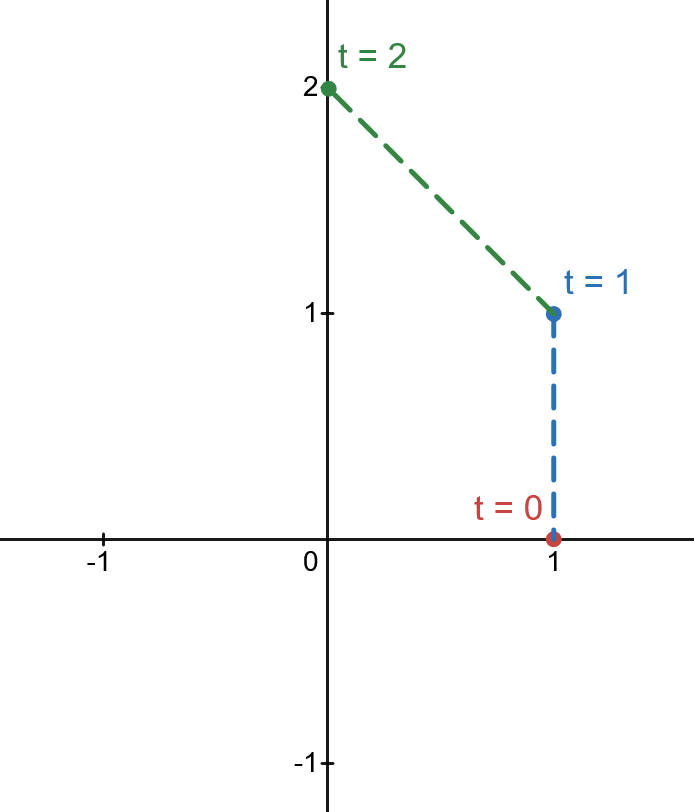
\includegraphics[width=0.8\textwidth]{section12_q2_1_fig.png}
\end{center}
\item The improved Euler's method has second order convergence ($p = 2$). We can use the same Lipschitz bound $L = 1$. The only constant that might change is $C$. Here the error given by the improved Euler's method will be upper bounded by $\frac{h}{6}\hat{u}''' + O(h^3)$. Again, we can give the crude upper bound of $C = 1$ and get an approximation of the global error by:
$$\|\hat{u}(t_i) - u_i\|_\infty \leq h^2\left[e^{\left\|t_i - \begin{bmatrix*}0 \\ 0\end{bmatrix*}\right\|_{\infty}} - 1\right].$$

Our approximation of $u$ from the two steps of improved Euler's method:
\begin{align*}
    k_1 &= hf(t_0, u_0) \\
    &= (1)\begin{bmatrix*}0 & -1 \\ 1 & 0\end{bmatrix*}\begin{bmatrix*}x(0) \\ y(0)\end{bmatrix*} \\
    &= (1)\begin{bmatrix*}0 & -1 \\ 1 & 0\end{bmatrix*}\begin{bmatrix*}1 \\ 0\end{bmatrix*} \\
    &= \begin{bmatrix*}0 \\ -1\end{bmatrix*} \\
    k_2 &= hf\left(t_0 + \frac{1}{2}h, u_0 + \frac{1}{2}k_1\right) \\
    &= (1)\begin{bmatrix*}0 & -1 \\ 1 & 0\end{bmatrix*}\left(\begin{bmatrix*}1 \\ 0\end{bmatrix*} + \frac{1}{2}\begin{bmatrix*}0 \\ -1\end{bmatrix*}\right) \\
    &= \begin{bmatrix*}\frac{1}{2} \\ 1\end{bmatrix*} \\
    \begin{bmatrix*}x(1) \\ y(1)\end{bmatrix*} &= \begin{bmatrix*}x(0) \\ y(0)\end{bmatrix*} + k_2 \\
    &= \begin{bmatrix*}1 \\ 0\end{bmatrix*}+ \begin{bmatrix*}\frac{1}{2} \\ 1 \end{bmatrix*}\\
    &= \begin{bmatrix*}\frac{3}{2} \\ 1\end{bmatrix*} \\
    k_1 &= (1)\begin{bmatrix*}0 & -1 \\ 1 & 0\end{bmatrix*}\begin{bmatrix*}\frac{3}{2} \\ 1\end{bmatrix*} \\
    &= \begin{bmatrix*}-1 \\ \frac{3}{2}\end{bmatrix*} \\
    k_2 &= hf\left(t_1 + \frac{1}{2}h, u_1 + \frac{1}{2}k_1\right) \\
    &= (1)\begin{bmatrix*}0 & -1 \\ 1 & 0\end{bmatrix*}\left(\begin{bmatrix*}\frac{3}{2} \\ 1\end{bmatrix*} + \frac{1}{2}\begin{bmatrix*}-1 \\ \frac{3}{2}\end{bmatrix*}\right) \\
    &= \begin{bmatrix*}0 & -1 \\ 1 & 0\end{bmatrix*}\begin{bmatrix*}1 \\ \frac{7}{4}\end{bmatrix*} \\
    &= \begin{bmatrix*}-\frac{7}{4} \\ 1\end{bmatrix*} \\
    \begin{bmatrix*}x(2) \\ y(2)\end{bmatrix*} &= \begin{bmatrix*}x(1) \\ y(1)\end{bmatrix*} + k_2 \\
    &= \begin{bmatrix*}\frac{3}{2} \\ 1\end{bmatrix*} + \begin{bmatrix*}-\frac{7}{4} \\ 1\end{bmatrix*} \\
    &= \begin{bmatrix*}-\frac{1}{4} \\ 2\end{bmatrix*}
\end{align*}
\begin{center}
    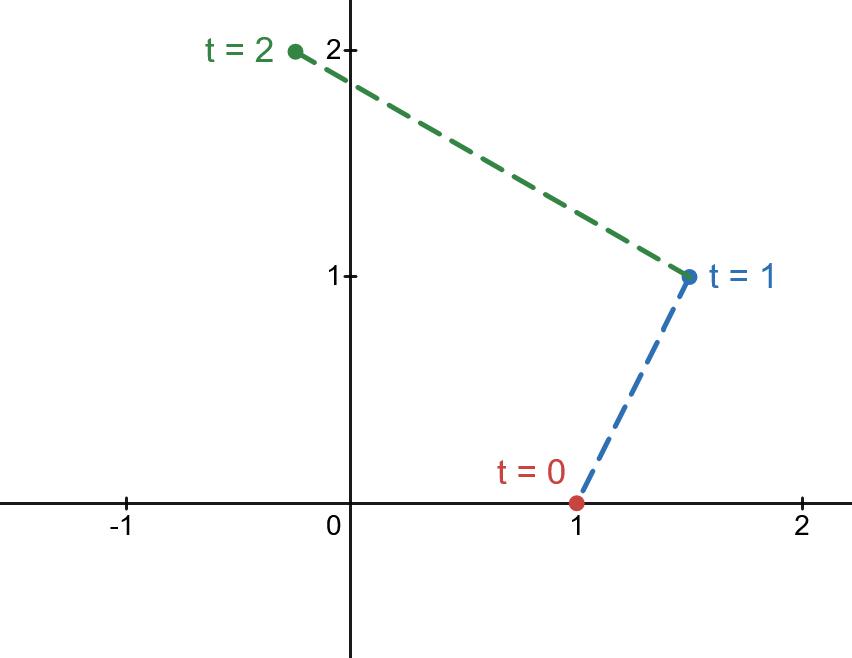
\includegraphics[width=0.8\textwidth]{section12_q2_2_fig.png}
\end{center}
\end{enumerate}
\end{solution}

\end{document}
